\section{Results}



\subsection*{In-the-loop flight tests}

\cref{fig:npjr_overview} gives an overview of our proposed system. We integrate an event camera and small recurrent convolutional neural network running on an on-board GPU into the drone's flight control loop. The network estimates attitude and rotation rates from event camera data with low latency, acting as a stand-in replacement of a regular IMU (inertial measurement unit), and allowing for accurate control. In traditional flight control loops, IMUs measuring linear accelerations and rotation rates are sampled at high frequency (typically 1~kHz or higher). These measurements are subsequently integrated in a Kalman or complementary filter running at a lower frequency (100-200 Hz) to produce accurate attitude and rotation rate estimates while filtering out the high-frequency noise produced by the sensors.

The proposed system instead uses data from an event camera in combination with a learned estimator. Events are accumulated into frames of 5~ms, and fed to a recurrent convolutional neural network that then estimates attitude and rotation rate. These estimates are then used by the angle and rate controller to compute desired thrust and torque, which are sent back to the flight controller at 200~Hz, and which are used for controlling the drone. We train our network through supervised learning on a dataset containing events, along with attitude and rotation rate estimates from the flight controller as labels. While these are not absolute ground truth (they are estimated by the flight controller using the IMU and can have bias), they are typically reliable enough.

\begin{figure}[t]
    \centering
    \includegraphics[width=\linewidth]{04_chapters/NPJR25/images/hover_plot.pdf}
    \caption{In-the-loop hover (position hold) flight tests with the network in control in the CyberZoo environment. The right-most time-lapse image shows the variation of the drone during flight, demonstrating the controllability of the drone over a total of approx. 10 minutes of flight time. The other plots quantify the errors of the estimated attitude and rotation rate for roll (rate) $\phi$ ($\dot{\phi}$) and pitch (rate) $\theta$ ($\dot{\theta}$). The ground truth (GT) angles and rates are measured by a motion capture system. The histograms give the error distribution of the network estimate compared to ground truth, with the biases of both subtracted (to disregard biases in training data). The left-most plots show the network errors for different attitude/rate combinations. These show that the network for both attitude and rate underestimates the real value. The bottom traces show the transition from IMU to network control, with a reset of the flight controller's integrator causing a short response of the drone before settling.}
    \label{fig:npjr_network_hover}
\end{figure}

The results from several flight tests with the trained network in the loop are shown in \cref{fig:npjr_network_hover}. For these tests, the pilot commands the drone to hold its position (hover), which the flight controller translates to attitude setpoints with the help of a higher-level position controller and a velocity sensor.\footnote{In our case, an optical flow sensor provided the velocity feedback used for position control. However, this outer-loop role could also have been fulfilled by the human pilot manually correcting position drift; we used the optical flow sensor instead to make the tests more repeatable and consistent.} These attitude setpoints are subsequently compared against estimates provided by the neural network. This results in desired rotation rates, which are also compared against network estimates, resulting in desired torques sent to the motors.

The traces and histograms show that the network can accurately estimate both attitude and rotation rate, with most errors within $\pm3$~deg and $\pm18$~deg/s for approx. 10 minutes of flight. The error plots for different attitude/rate combinations show that most errors are due to underestimation by the network, which can also be seen in the difference between network and ground truth during the transition phase. Underestimation is most pronounced at high angles/rotation rates, which could be explained by the inertia of the network's memory. While this allows integration of information over time, it also limits the network in following fast maneuvers.

The error histograms further reveal axis-dependent asymmetries: attitude estimates are more accurate for roll than for pitch, whereas the opposite holds for rotation rate estimates. We attribute reduced accuracy in pitch attitude estimation primarily to limited pitch-angle variability during training and minor shifts in drone balance along the pitch axis (such as varying battery position). Conversely, the decreased accuracy observed in roll rate predictions aligns with the larger amounts of oscillation around the roll axis.

\cref{fig:npjr_network_square} shows flight tests with more dynamic maneuvers in two environments: CyberZoo (training environment) and Factory. The pilot controls the drone to fly an approximate square. The plots show that the network estimates of the angle and rotation rate are accurate for the most part. While the network, especially in the case of Factory, sometimes underestimates the roll angle, the rotation rate estimates are very good, which is most important for controllable flight. The bottom row of plots compares the angle estimates of the flight controller with the angles desired following the pilot's inputs. It is clearly visible that the controller manages to track the given commands. 

\begin{figure}[t]
    \centering
    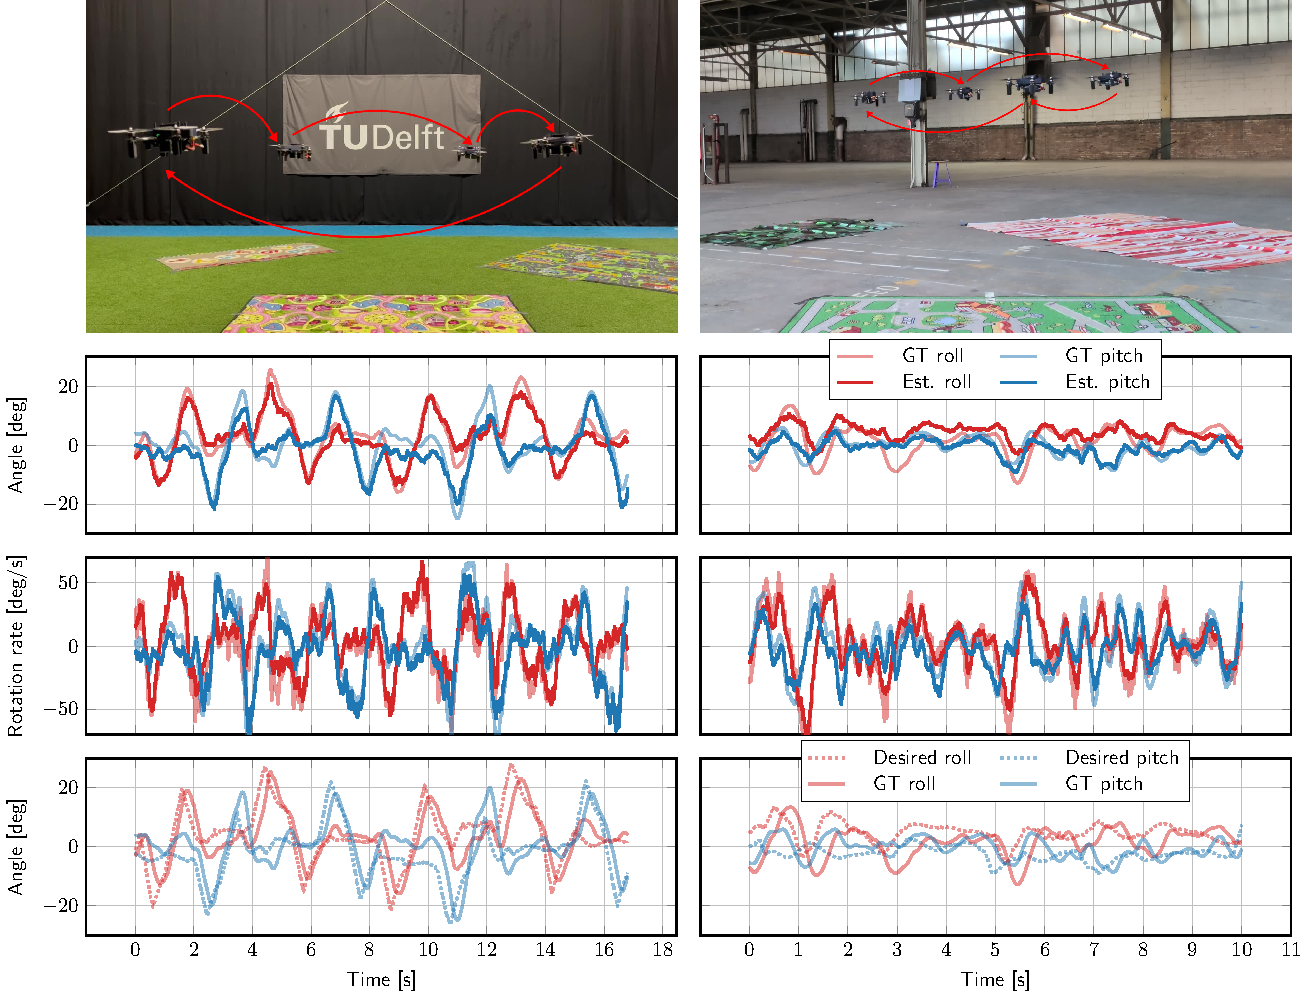
\includegraphics[width=\linewidth]{04_chapters/NPJR25/tikz/externalized/tikz-figure1.pdf}
    \caption{In-the-loop flight tests with the network in control in two different environments: CyberZoo (left) and Factory (right). The pilot manually controls the drone to fly an approximate square (note that the square for Factory is smaller). The first row of plots shows estimated (from the network) versus ground-truth (from motion capture for CyberZoo, from flight controller for Factory) roll and pitch angles of the drone. The second row shows the angular rate estimates. These demonstrate how well the network can estimate angles and angular rates based on vision. The third row shows the angle estimates by the network again, but now compared against the angles that were desired to follow the pilot's input. This shows how usable the estimates by the network are for controlling the drone.}
    \label{fig:npjr_network_square}
\end{figure}





\subsection*{Comparison of models}

We conducted an extensive comparison of neural network models with varying network architecture, input modalities and input resolution. \cref{tab:npjr_results} lists the performance of these variations in terms of RMSE (root mean square error) and MASD (mean absolute successive difference) when tested on unseen data from the training environment. While RMSE gives a good measure of the estimation error, MASD quantifies prediction smoothness by looking at the difference between subsequent predictions. A qualitative illustration of the estimation performance of various neural networks is given in \cref{fig:npjr_network_traces}.

The baseline, \textit{Vision}, receives only event frames as input and processes these with a convolutional neural network with GRU (gated recurrent unit) memory block. This variant was used for the in-control flight tests in \cref{fig:npjr_network_hover,fig:npjr_network_square}. \textit{VisionMotor} additionally takes motor speeds as input. These can serve as a proxy for the moment generated by the motors, (a prediction of) which was shown to be necessary for the attitude to be observable~\cite{decroon2022accommodating}. In our learning setup, however, the error difference with the vision-only model is small: only the estimation of rotation rates is slightly better, which makes sense given that the forces produced by the motors can be integrated to obtain rotational velocities. \textit{VisionGyro} receives gyro measurements (rotation rates) as additional inputs. This represents the case in which a gyro would still be present in the system, and its performance can give an idea of whether the network could integrate rotation rate to obtain the attitude. As expected, this results in the lowest-error rotation rate estimates. The accuracy of the attitude prediction, however, is not meaningfully better.
\textit{VisionFF} replaces the recurrent memory block with a feedforward alternative, and will therefore not be able to integrate information over time. While attitude can be inferred from a single image by looking at horizon-like visual cues (such as those indicated by the white arrows in \cref{fig:npjr_motionmodel}), the increased attitude error of \textit{VisionFF} compared to \textit{Vision} suggests that having memory is still beneficial. Estimation of velocities such as rotation rate is very difficult without memory, and this is reflected by the large increase in rotation rate error. 

\textit{VisionSNN} is a hybrid spiking neural network (SNN) where the encoder has binary activations (stateless spiking neurons) and the recurrent memory block consists of spiking LIF (leaky integrate-and-fire) neurons with a recurrent connection. While the quantitative errors for \textit{VisionFF} and \textit{VisionSNN} are similar, \cref{fig:npjr_network_traces} shows that the SNN's memory makes a difference for estimating rotation rates.











\begin{sidewaysfigure}[htbp]
  \centering
  \begin{minipage}[c]{0.29\textwidth}
    \centering
    \includegraphics[width=\linewidth]{04_chapters/NPJR25/images/network_traces.pdf}
    \caption{Qualitative comparison of attitude and rotation rate estimates for various neural network architectures on unseen data from the training environment. The network variants match those in \cref{tab:npjr_results}. Ground truth (GT) is coming from the flight controller estimate.}
    \label{fig:npjr_network_traces}
  \end{minipage}
  \hfill
  \begin{minipage}[c]{0.69\textwidth}
    \centering
    \begin{tabular}{lrrrr}
      \toprule
                  & \multicolumn{2}{c}{Attitude}    & \multicolumn{2}{c}{Rotation rate} \\ 
      \cmidrule(l){2-5} 
      Network     & RMSE {[}deg{]} & MASD {[}deg{]}  & RMSE {[}deg/s{]}  & MASD {[}deg/s{]}   \\ 
      \midrule
      Vision      & \underline{1.51}    & \textbf{0.27} & 10.65          & 2.57           \\
      VisionMotor & 1.64          & \underline{0.31}          & \underline{9.57}     & \underline{2.47}     \\
      VisionGyro  & \textbf{1.47} & \underline{0.31}    & \textbf{4.01}  & \textbf{2.36}  \\
      VisionFF    & 2.17          & 1.00          & 18.65          & 5.82           \\
      VisionSNN   & 2.17          & 0.52          & 15.03          & 4.04           \\ 
      \bottomrule
    \end{tabular}
    \captionof{table}{Performance of models with different network architectures and inputs on unseen data from the training environment. \textit{Vision} is the baseline model with ConvGRU memory and vision-only input. \textit{VisionMotor} additionally has motor commands as input. \textit{VisionGyro} receives gyro measurements as additional input. \textit{VisionFF} has a memory-less architecture (feedforward). \textit{VisionSNN} is a hybrid spiking neural network. We quantify performance in terms of RMSE (root mean square error) and MASD (mean absolute successive difference) with the flight controller estimates as ground truth.}
    \label{tab:npjr_results}
  \end{minipage}
\end{sidewaysfigure}



Next, we investigate the impact of varying input resolution. Under rapid motion, event cameras generate a large amount of events, which can lead to bandwidth saturation and increased latency when working with on-board, constrained hardware. The event camera used in this work, a DVXplorer Micro, allows disabling pixels to limit the number of events generated by the camera. \cref{fig:npjr_resolution_comp} analyzes the impact of using lower-resolution data on network performance when training with otherwise identical settings. Apart from quantifying the estimation error using RMSE, we also look at the prediction delay of the network. When actively controlling a system, significant delays lead to oscillations and potentially instability, and should therefore be avoided. We quantify the prediction delay of each network by looking at the time shift for which the Pearson correlation coefficient (PCC) is lowest. The results show that there is a noticeable delay in predictions when using only a quarter of the camera's pixels. We attribute this to the fact that attitude changes might only be seen by any of the enabled pixels once they become large enough, leading to a delayed response. This delay is much less present for half and full-resolution networks. Interestingly, the full-resolution network shows a slightly higher attitude RMSE compared to the half-resolution network. This could be explained by the fact that all networks were trained for the same number of epochs, whereas the larger full-resolution network likely requires more training steps before achieving similar convergence. The half-resolution network brings a good balance between computational efficiency and estimation performance.



\begin{figure}[h!]
    \centering
    \includegraphics[width=\linewidth]{04_chapters/NPJR25/images/resolution_comp.pdf}
    \caption{The impact of resolution on network performance after training under otherwise identical settings. Results were obtained by enabling only a subset of event camera pixels: every fourth pixel (quarter resolution, blue), every other pixel (half resolution, orange) and all pixels (full resolution, green). The bottom-left graphs show the PCC (Pearson correlation coefficient) for different time shifts of the prediction targets. The minimum of each line indicates the shift with the highest correlation. Minima at larger shifts indicate a delay in the network prediction. The bottom-right plots show the RMSE (root mean square error) on validation data. We use the flight controller estimates as ground truth. Networks trained on quarter-resolution data show larger prediction delay and increased error compared to higher resolutions.}
    \label{fig:npjr_resolution_comp}
\end{figure}


\subsection*{Generalization and internal motion model}


Recent work~\cite{decroon2022accommodating} has shown that attitude can be inferred from optical flow when combined with a motion model relating attitude to acceleration direction. While the learning framework presented here does not explicitly represent such a model internally, it would be interesting to investigate whether this can be promoted during learning, and whether this affects generalization to different scenes. In other words, we would like to steer the network towards using optical flow for attitude estimation, instead of static visual cues such as horizon-like straight lines on the edges of the field of view (indicated by white arrows on the right in \cref{fig:npjr_motionmodel}). We hypothesize that networks that rely mainly on motion features generalize better across environments than networks that focus on visual appearance, which is more scene-specific and may lead to overfitting on the training scene.

To achieve this, we trained a network on the same dataset as before (CyberZoo), but restricted its input to a small 160$\times$120 center crop. This eliminates most visual cues that contain absolute attitude information while preserving motion cues. We refer to the original, unrestricted model as \textit{full FoV} (identical to \textit{Vision} from \cref{tab:npjr_results}) and the newly trained variant as \textit{center crop}. We evaluate these models on four unseen sequences, and show the results in \cref{fig:npjr_motionmodel}. The full-FoV network effectively makes use of the horizon-like cues present in most sequences (white arrows for CyberZoo, Office and Outdoor), generalizing well to other scenes and outperforming the center-crop model. However, we also include a sequence from the event camera dataset ECD \texttt{poster\_rotation} recording~\cite{mueggler2017eventcamera}. Here, a camera (different from ours) looks at a planar poster while undergoing rotations, without any visual cues related to the camera's attitude. On this sequence, the center-crop network achieved lower attitude and rate errors than the full-FoV network. This indicates that the center-crop network can effectively use motion information to infer attitude, hinting at an internally acquired motion model. Furthermore, looking at the relative error across environments, we see that relative error increases less for the center-crop network when moving from the familiar training environment to novel scenes. This presents a trade-off: while networks with access to the full FoV have better absolute performance for scenes with horizon-like visual cues, networks forced to infer attitude from motion through a reduced FoV relatively generalize better across environments. If we remove memory from the network (\textit{center crop + feedforward}), it performs poorly for both attitude and rotation rate estimation. Such a network has neither the field of view for static attitude information, nor the ability to build it up through memory.



\begin{figure}[h!]
    \centering
    \includegraphics[width=\linewidth]{04_chapters/NPJR25/images/motion_model_results_with_images.pdf}
    \caption{Comparison between a network with memory and full field-of-view (baseline), a network with memory that only sees a center-cropped portion (indicated by the white rectangle), and a network without memory that only sees a center-cropped portion. We compare estimation errors for four unseen sequences, with the flight controller's estimate as ground truth. CyberZoo is the same environment as trained on, but Office, Outdoor and ECD \texttt{poster\_rotation} (rotation only)~\cite{mueggler2017eventcamera} are unseen environments. While the full-FoV network performs better in scenes where horizon information (indicated by white arrows) is available to provide an absolute indication of attitude (CyberZoo, Office, Outdoor), the center-cropped network performs better when there are no visible horizon-like cues (as in ECD \texttt{poster\_rotation}), hinting at the use of an internal motion model. Additionally, the smaller relative increase in error in the case of the center-cropped network for scenes different from the training location CyberZoo indicates improved generalization. A memory-less center-crop network is unable to aggregate information internally into any kind of model, and hence performs poorly in terms of both attitude and rotation rate estimation.}
    \label{fig:npjr_motionmodel}
\end{figure}
